%% The following is a directive for TeXShop to indicate the main file
%%!TEX root = diss.tex

\chapter{Background}
\label{ch:background}

\section{IoT Architecture}
Figure \autoref{fig:arch} shows a typical architecture of an IoT system~\citep{towardsIoTDefinition,stojkoska2017review,vcolakovic2018IoT,eclipse2016three}. 

\subsection{Device Layer}
The device layer at the bottom, which is the closest component to the physical world, includes smart programmable things interacting with the environment through their embedded sensors and actuators. Some IoT devices employ light embedded operating systems (e.g. contiki, RIOT, TinyOS) that have support for various programming languages allowing developers to write embedded code, such as application-specific logics for devices, on top of the device OS~\cite{javed2018OS}. IoT operating systems aim to hide the minor details of the device hardware and provide basic OS tasks, like memory management and real-time scheduling, efficiently\cite{javed2018OS}. On the other side of spectrum, bare metal IoT devices run the embedded code directly on their hardware processor. Underlying details of the device hardware is usually abstracted by hardware abstraction layer (HAL) to enable access for the operating system to various hardware components like GPIO, and serial interfaces\cite{eclipse2016three}. In addition, IoT devices should have a connectivity capability which includes drivers, external libraries, and communication protocols to allow them communicate over a local wired or wireless communication.

There are different types of IoT devices based on their processing, power, and storage capabilities~\cite{bormann2014terminology} which affects the way they communicate with the cloud systems over the internet. Gateway-connected devices, as the name suggested in~\cite{securityUsenix2019}, are designed to do a limited functionality due to their constrained resources, thus, they rely on gateway devices for specific application purposes, data management, or secure communication with remote cloud systems~\cite{bormann2014terminology}. On the other hand, cloud-connected devices have the ability to talk directly to the cloud by employing protocols designed specifically for constrained devices like Constrained Application Protocol (CoAP). They should have enough resources to do basic data pre-processing and to apply security mechanisms by themselves without the help of a gateway device~\cite{stojkoska2017review,securityUsenix2019}. In addition, both types of IoT devices allow higher level components to control, monitor, and upgrade them remotely~\cite{eclipse2016three}.


 \begin{figure}[t]
  \centering 
   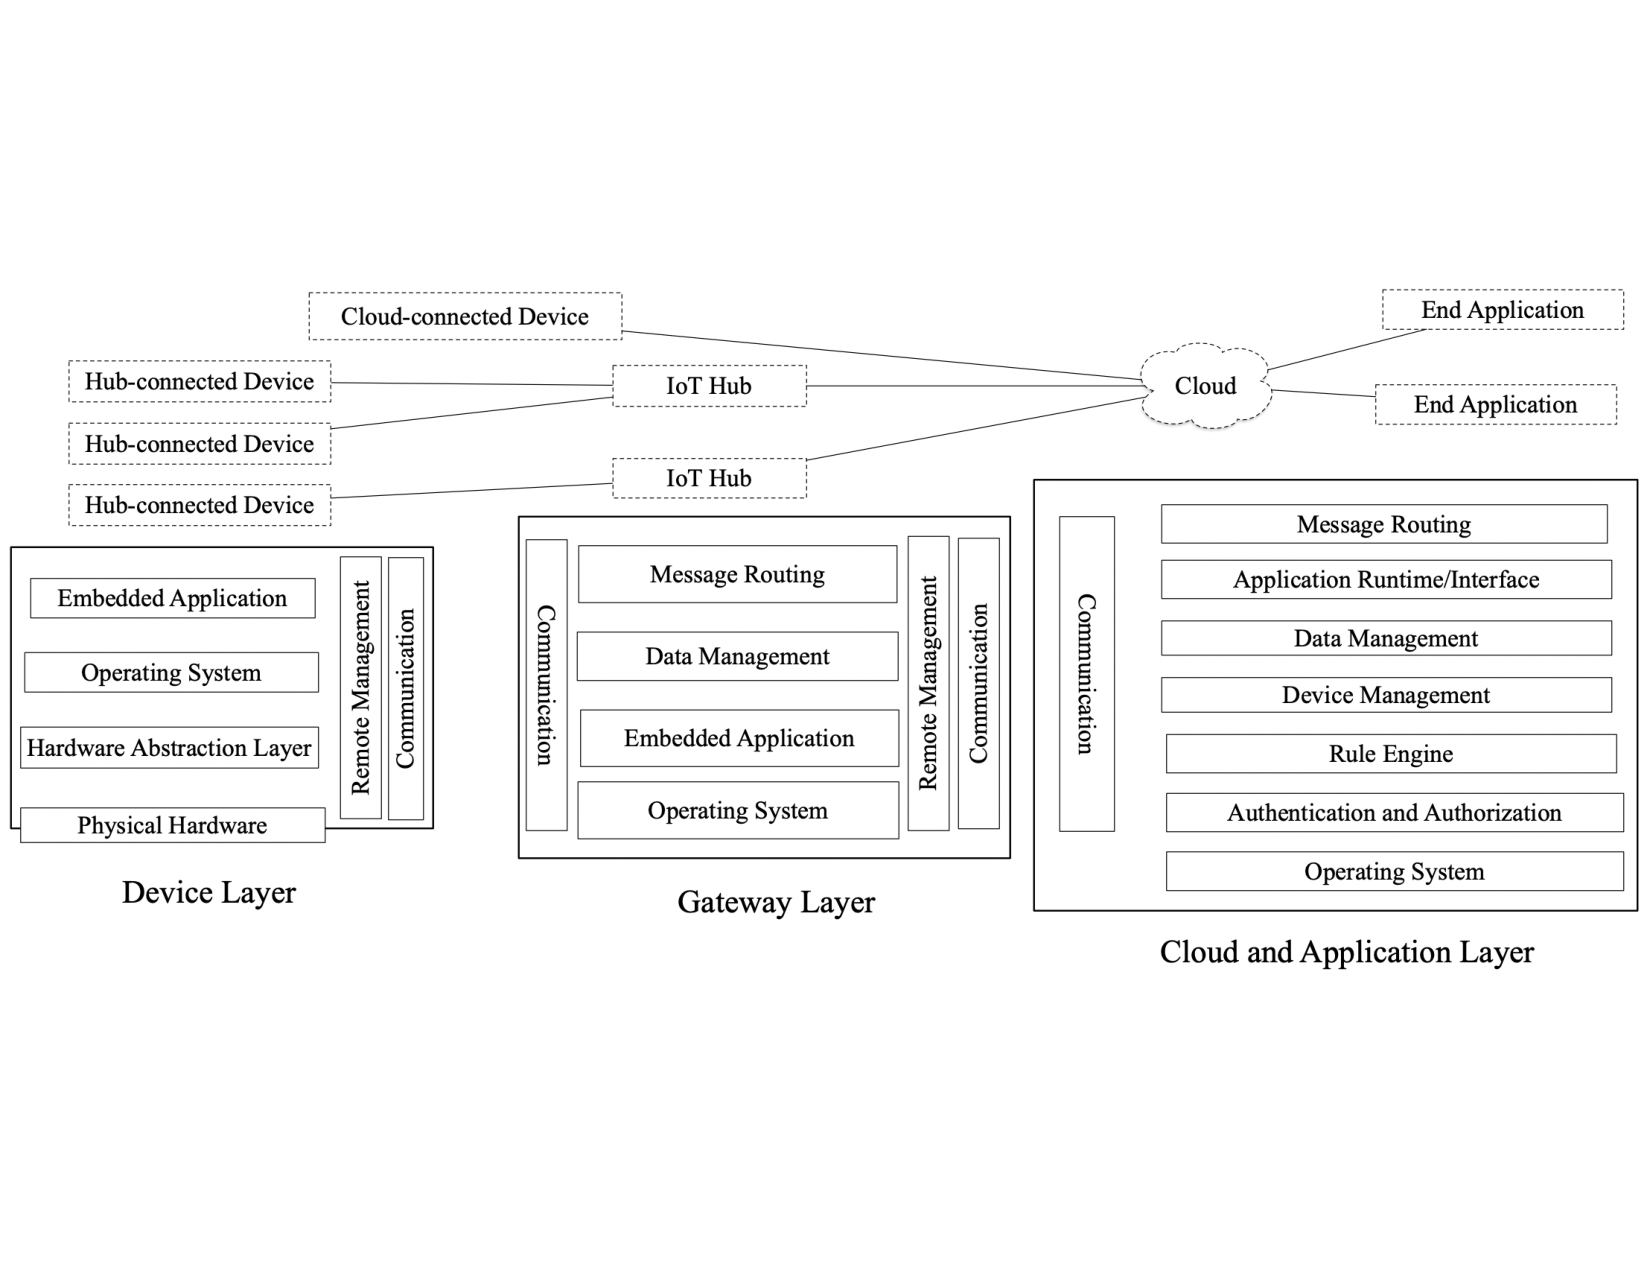
\includegraphics[width=\linewidth]{./imgs/arch1.pdf}
  \caption{A typical layered architecture of IoT systems and software stack for each layer}
  \label{fig:arch}
\end{figure}

\subsection{Gateway Layer}
This layer contains gateway devices with fewer resource constraints with the ability to handle telemetry data collection, processing, and routing locally on the edge. Gateway devices can handle the device-device and device-cloud interoperability by interpreting diverse communication protocols such as MQTT, CoAP, and HTTP~\cite{tschofenig2014architectural}. 

The IoT gateway devices have less resource constraint and the ability to handle telemetry data collection, processing, and routing locally on the edge. These devices can offer secure communication with remote systems since they can employ full-stack communication protocols and security mechanisms\cite{bormann2014terminology}. Gateway devices can handle the device-device and device-cloud interoperability by interpreting diverse communication protocols of both sides\cite{vcolakovic2018IoT}.

\subsection{Cloud and Application Layer}
Remote IoT cloud servers accumulate and process all telemetry data, and communicate with heterogeneous IoT devices to control and monitor them remotely. IoT cloud servers rule engine lets users write automation logic between IoT devices to define interoperability behaviours of the IoT system~\cite{securityUsenix2019}. 

The most advanced and complex part of the IoT architecture is the remote cloud servers \cite{stojkoska2017review}where all the data are accumulated and processed. Cloud servers can communicate with large number of heterogeneous gateway or cloud-connected devices at the same time. Users can monitor the telemetry data and device status, and send commands to IoT devices to control and configure them remotely from the cloud. End users should be authenticated and authorized in the cloud to be able to use these services. Cloud systems usually have a rule engine which let users write custom logic and automation between IoT devices to define interoperability behaviours of the IoT system \cite{securityUsenix2019}. Cloud systems can offer their own analytic, dashboard and visualization services to end-users, provide interface for third-party applications, and allow users to run custom code in the application runtime environment on top of the cloud services\cite{vcolakovic2018IoT}.

Some IoT systems offer specific services to end-users, provide interface for third-party applications, and allow users to run custom code in the application runtime environment on top of their services\cite{vcolakovic2018IoT}.






\endinput

